%%%%%%%%%%%%%%%%%%%%%%%%%%%%%%%%%%%%%%%%%%%%%%%%%%%%%%%%%%%
% Two-page research showcase followed by the technical report template.
% Replace every [TO COMPLETE] marker and framed placeholder as the
% calculation is validated. Set \reportdraftfalse before submission.
%%%%%%%%%%%%%%%%%%%%%%%%%%%%%%%%%%%%%%%%%%%%%%%%%%%%%%%%%%%

\documentclass[9pt,a4paper,twocolumn,twoside]{rho-class/rho}
\usepackage[english]{babel}
\usepackage{amsmath}

%----------------------------------------------------------
% Draft helpers
%----------------------------------------------------------

\newif\ifreportdraft
\reportdrafttrue

\newcommand{\draftnote}[1]{%
    \ifreportdraft
        \par\smallskip
        \noindent\textbf{\textsf{[TO COMPLETE]}} \textit{#1}
        \par\smallskip
    \fi
}

\newcommand{\figureplaceholder}[2][38mm]{%
    \begingroup
    \setlength{\fboxsep}{5pt}%
    \fbox{%
        \parbox[c][#1][c]{0.91\linewidth}{%
            \centering\small\textsf{FIGURE PLACEHOLDER}\par\medskip
            #2
        }%
    }%
    \endgroup
}

\newcommand{\ac}{a_{\mathrm{c}}}
\newcommand{\abg}{a_{\mathrm{bg}}}
\newcommand{\Jmol}{\mathcal{J}_{\mathrm{m}}}
\newcommand{\Rsm}{\mathcal{R}_{\mathrm{sm}}}
\newcommand{\dd}{\mathrm{d}}
\newcommand{\ii}{\mathrm{i}}

%----------------------------------------------------------
% Showcase-page styling
%----------------------------------------------------------

\definecolor{showcasenavy}{HTML}{143D66}
\definecolor{showcaseblue}{HTML}{2474A6}
\definecolor{showcasecyan}{HTML}{69AEC9}
\definecolor{showcasered}{HTML}{B6403A}
\definecolor{showcasegold}{HTML}{D49A22}
\definecolor{showcaseink}{HTML}{27313D}
\definecolor{showcasemist}{HTML}{EEF5F8}

\newcommand{\showcaseheading}[1]{%
    {\color{showcasenavy}\sffamily\bfseries\fontsize{15}{17}\selectfont #1\par}%
    \vspace{2mm}%
}

\newcommand{\showcasesubheading}[1]{%
    {\color{showcasenavy}\sffamily\bfseries\fontsize{11}{13}\selectfont #1\par}%
    \vspace{1.2mm}%
}

\tcbset{
    showcasebox/.style={
        enhanced,
        colback=showcasemist,
        colframe=showcaseblue,
        boxrule=0.7pt,
        arc=3pt,
        left=4mm,
        right=4mm,
        top=3mm,
        bottom=3mm,
        fontupper=\sffamily,
        before upper=\RaggedRight,
    },
    showcasecard/.style={
        enhanced,
        colback=white,
        colframe=showcasecyan!65,
        boxrule=0.6pt,
        arc=3pt,
        left=2.5mm,
        right=2.5mm,
        top=2.5mm,
        bottom=2.5mm,
        fontupper=\sffamily,
        before upper=\RaggedRight,
    },
}

\fancypagestyle{showcasestyle}{%
    \fancyhf{}%
    \renewcommand{\headrulewidth}{0pt}%
    \renewcommand{\footrulewidth}{0pt}%
}

%----------------------------------------------------------
% Title and front matter
%----------------------------------------------------------

\doctype{Final Research Report}
\title{Optimal Laser-Constrained Control of Molecular Formation from a Quantum Gas via Optical Feshbach Resonances}

\author{Charlie Mullen}
\affil{Department of Physics, The Chinese University of Hong Kong}

\corres{\textsuperscript{*}Student author: Charlie Mullen. Supervisor: Prof. Yangqian Yan.}
\docinfo{IASP 4090 Independent Research on International Studies, Summer Undergraduate Research Programme. \ifreportdraft\textbf{Draft boilerplate:} replace all marked prompts before submission.\fi}

\journalname{CUHK SURP}
\journal{IASP 4090 Final Research Report}
\theday{\today}

%----------------------------------------------------------
% Abstract and keywords
%----------------------------------------------------------

\begin{abstract}
    Optical Feshbach resonances provide a fast, species-flexible means of controlling ultracold interactions, but the same optical coupling that changes the real scattering length also opens an inelastic molecular channel. This report develops a numerical optimal-control framework for maximizing the molecular yield accumulated over a fixed time while respecting a finite laser-intensity budget. The physical controls are the dimensionless stimulated linewidth and detuning, which jointly determine a complex scattering length. Their history drives a universal short-time pair amplitude through a half-order Volterra equation, and the loss--contact relation converts that amplitude into a molecular production rate. The resulting constrained objective is optimized with automatically differentiated, GRAPE-style piecewise controls and translated to the $689$-nm $^1S_0$--$^3P_1$ optical Feshbach resonance of bosonic $^{88}\mathrm{Sr}$. The archived $N=100$ multi-start result shown here is provisional; the absolute yield normalization, time-grid convergence, cap sweep, and laboratory prescription remain to be validated.
\end{abstract}

\keywords{optical Feshbach resonance, ultracold quantum gas, Tan contact, molecular formation, optimal control, Volterra equation, JAX}

%----------------------------------------------------------

\begin{document}

%==========================================================
% RESEARCH SHOWCASE — PAGE 1
%==========================================================

\newgeometry{left=1.15cm,right=1.15cm,top=0.9cm,bottom=0.9cm}
\onecolumn
\pagestyle{showcasestyle}
\thispagestyle{showcasestyle}

\begin{tcolorbox}[
    enhanced,
    colback=showcasenavy,
    colframe=showcasenavy,
    boxrule=0pt,
    arc=4pt,
    left=7mm,
    right=7mm,
    top=5mm,
    bottom=5mm
]
    {\color{showcasecyan!65!white}\sffamily\bfseries\fontsize{9}{11}\selectfont
    CUHK SUMMER UNDERGRADUATE RESEARCH PROGRAMME \hfill RESEARCH SHOWCASE}

    \vspace{2mm}
    {\color{white}\sffamily\bfseries\fontsize{27}{30}\selectfont
    Shaping quantum collisions with light\par}
    \vspace{1mm}
    {\color{white!90}\sffamily\fontsize{14}{17}\selectfont
    Optimal laser control of molecule formation through an optical Feshbach resonance\par}
    \vspace{3mm}
    {\color{white}\sffamily\fontsize{9}{11}\selectfont
    \textbf{Charlie Mullen} \enspace|\enspace Supervisor: Prof. Yangqian Yan
    \hfill Department of Physics, The Chinese University of Hong Kong}
\end{tcolorbox}

\vspace{3mm}
\begin{tcolorbox}[showcasebox,colback=showcasegold!12,colframe=showcasegold]
    \begin{minipage}[c]{0.17\textwidth}
        {\color{showcasegold!75!black}\sffamily\bfseries\fontsize{11}{13}\selectfont
        \mbox{THE QUESTION}}
    \end{minipage}\hfill
    \begin{minipage}[c]{0.79\textwidth}
        {\color{showcaseink}\sffamily\bfseries\fontsize{14}{17}\selectfont
        Can a laser assemble molecules from an ultracold gas without simply destroying the atoms?}
    \end{minipage}
\end{tcolorbox}

\vspace{3mm}
\begin{minipage}[t]{0.385\textwidth}
    \vspace{0pt}
    \showcaseheading{The problem in plain language}
    {\sffamily\fontsize{10.2}{13.1}\selectfont
    At a few billionths of a degree above absolute zero, atoms behave as coherent matter waves. A laser tuned near a molecular resonance can change how two waves scatter---and can briefly couple an atom pair to a molecular state.

    \vspace{2.2mm}
    That opportunity comes with a cost: the excited molecule can decay. The useful interaction and the unwanted loss are two parts of the same \emph{complex scattering length}. Turning the intensity up does not provide an independent ``molecule knob.''

    \vspace{2.2mm}
    The gas also remembers. The rate at one instant depends on pair correlations built by the entire earlier pulse, so the best control is a time sequence rather than one fixed laser setting.}

    \vspace{3mm}
    \begin{tcolorbox}[showcasecard,colframe=showcasered!65,colback=showcasered!5]
        \showcasesubheading{The central trade-off}
        {\sffamily\fontsize{9.2}{11.6}\selectfont
        Detuning from resonance reduces decay, but also weakens the interaction. Intensity strengthens both. The optimization must decide \textbf{when to build correlations} and \textbf{when to convert them into products}.}
    \end{tcolorbox}

\end{minipage}\hfill
\begin{minipage}[t]{0.585\textwidth}
    \vspace{0pt}
    \showcaseheading{One laser, two inseparable effects}
    \centering
    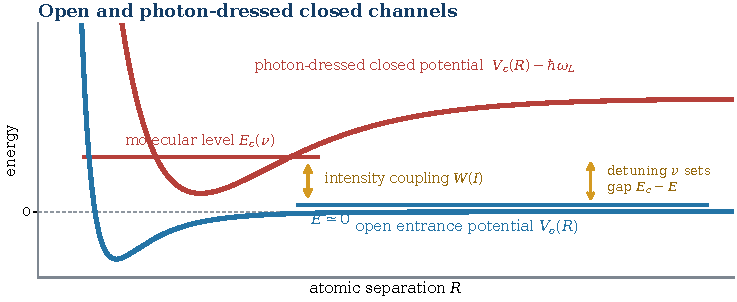
\includegraphics[width=0.98\linewidth]{figures/figure1_ofr_schematic.pdf}

    \vspace{1.5mm}
    \begin{tcolorbox}[showcasecard,colback=showcasemist,colframe=showcasecyan]
        {\raggedright\sffamily\fontsize{9.1}{11.4}\selectfont
        \textbf{Left:} the laser couples colliding atoms to an excited molecule; spontaneous decay opens a loss channel. \textbf{Right:} at fixed intensity, changing detuning moves the scattering length around a circle in the complex plane. Intensity selects the circle. The elastic and lossy responses therefore cannot be programmed independently.\par}
    \end{tcolorbox}

    \vspace{2mm}
    \begin{tcolorbox}[showcasecard,colframe=showcaseblue!65,colback=showcaseblue!5]
        \showcasesubheading{Why use $^{88}\mathrm{Sr}$?}
        {\sffamily\fontsize{9.2}{11.6}\selectfont
        Its narrow $689\,\mathrm{nm}$ intercombination transition enables optical control with a comparatively long-lived excited molecular state. Its background interaction is close to zero, so changes of only a few Bohr radii strongly affect the gas \cite{blatt2011measurement,yan2013controlling}.}
    \end{tcolorbox}
\end{minipage}

\vspace{3mm}
\showcaseheading{From two laser waveforms to one objective}
\begin{tcbraster}[
    raster columns=5,
    raster equal height=rows,
    raster column skip=2.4mm,
    raster row skip=0mm
]
    \begin{tcolorbox}[showcasecard,colframe=showcasegold]
        {\color{showcasegold!75!black}\bfseries\fontsize{13}{14}\selectfont 1}\par\smallskip
        {\bfseries Laser controls}\par
        \smallskip$\Gamma(t)$ sets coupling; $\nu(t)$ sets detuning.
    \end{tcolorbox}
    \begin{tcolorbox}[showcasecard,colframe=showcaseblue]
        {\color{showcaseblue}\bfseries\fontsize{13}{14}\selectfont 2}\par\smallskip
        {\bfseries Complex interaction}\par
        \smallskip$\ac(t)$ links elastic response and loss.
    \end{tcolorbox}
    \begin{tcolorbox}[showcasecard,colframe=showcasecyan]
        {\color{showcaseblue}\bfseries\fontsize{13}{14}\selectfont 3}\par\smallskip
        {\bfseries Quantum memory}\par
        \smallskip A Volterra equation evolves $\eta(t)$.
    \end{tcolorbox}
    \begin{tcolorbox}[showcasecard,colframe=showcaseblue]
        {\color{showcaseblue}\bfseries\fontsize{13}{14}\selectfont 4}\par\smallskip
        {\bfseries Correlated pairs}\par
        \smallskip Tan's contact scales as $|\eta(t)|^2$.
    \end{tcolorbox}
    \begin{tcolorbox}[showcasecard,colframe=showcasered]
        {\color{showcasered}\bfseries\fontsize{13}{14}\selectfont 5}\par\smallskip
        {\bfseries Molecular yield}\par
        \smallskip Accumulate the lossy pair flux over time.
    \end{tcolorbox}
\end{tcbraster}

\vspace{3mm}
\begin{tcolorbox}[
    enhanced,colback=showcaseblue,colframe=showcaseblue,boxrule=0pt,arc=3pt,
    left=5mm,right=5mm,top=3mm,bottom=3mm
]
    {\color{white}\sffamily\bfseries\fontsize{11}{14}\selectfont
    Strategy: use automatic differentiation to search smooth, bounded intensity and detuning histories---while retaining the memory of every earlier control decision.}
\end{tcolorbox}

\newpage

%==========================================================
% RESEARCH SHOWCASE — PAGE 2
%==========================================================

\thispagestyle{showcasestyle}
\noindent
\begin{minipage}[c]{0.76\textwidth}
    {\color{showcasenavy}\sffamily\bfseries\fontsize{24}{27}\selectfont
    What the calculation shows so far\par}
    \vspace{1mm}
    {\color{showcaseink}\sffamily\fontsize{11}{14}\selectfont
    A completed archived multi-start run provides a concrete pulse and a reproducibility check.}
\end{minipage}\hfill
\begin{minipage}[c]{0.20\textwidth}
    \begin{tcolorbox}[
        enhanced,colback=showcasegold!15,colframe=showcasegold,boxrule=0.7pt,
        arc=8pt,left=2mm,right=2mm,top=2mm,bottom=2mm
    ]
        \centering\color{showcasegold!65!black}\sffamily\bfseries
        PRELIMINARY\\[-1pt]
        {\fontsize{7.8}{9}\selectfont VALIDATION IN PROGRESS}
    \end{tcolorbox}
\end{minipage}

\vspace{3mm}
\begin{tcolorbox}[showcasebox,colback=white,colframe=showcasecyan,left=3mm,right=3mm,top=2mm,bottom=2mm]
    \centering
    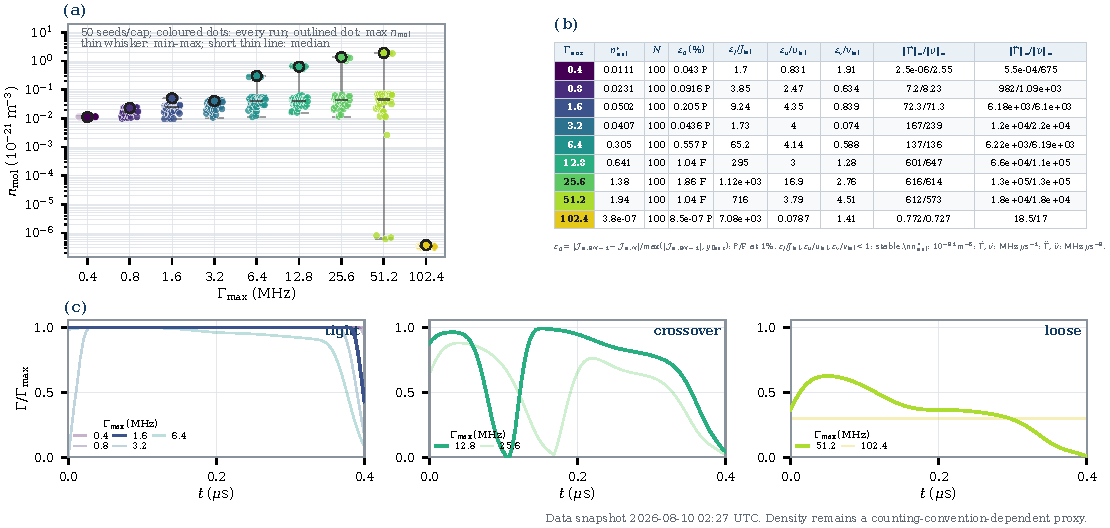
\includegraphics[width=0.99\linewidth]{figures/showcase_provisional_results.pdf}
\end{tcolorbox}

\vspace{3mm}
\begin{tcbraster}[
    raster columns=4,
    raster equal height=rows,
    raster column skip=2.5mm,
    raster row skip=0mm
]
    \begin{tcolorbox}[showcasecard,colframe=showcaseblue]
        \centering{\color{showcasenavy}\bfseries\fontsize{20}{22}\selectfont 40/40}\par
        \smallskip archived starts completed
    \end{tcolorbox}
    \begin{tcolorbox}[showcasecard,colframe=showcasecyan]
        \centering{\color{showcasenavy}\bfseries\fontsize{20}{22}\selectfont 25,000}\par
        \smallskip Adam steps per start
    \end{tcolorbox}
    \begin{tcolorbox}[showcasecard,colframe=showcasegold]
        \centering{\color{showcasenavy}\bfseries\fontsize{20}{22}\selectfont 23.8 ppm}\par
        \smallskip best-to-worst objective spread
    \end{tcolorbox}
    \begin{tcolorbox}[showcasecard,colframe=showcasered]
        \centering{\color{showcasenavy}\bfseries\fontsize{20}{22}\selectfont $N=100$}\par
        \smallskip provisional time grid
    \end{tcolorbox}
\end{tcbraster}

\vspace{4mm}
\begin{minipage}[t]{0.315\textwidth}
    \vspace{0pt}
    \begin{tcolorbox}[showcasecard,colframe=showcaseblue,colback=showcaseblue!4]
        \showcaseheading{How to read the pulse}
        {\sffamily\fontsize{9.1}{11.5}\selectfont
        \textcolor{showcaseblue}{\textbf{1. Couple strongly at first.}} The best archived intensity begins at the cap, then quickly drops.

        \vspace{2mm}
        \textcolor{showcasered}{\textbf{2. Chirp the detuning.}} The pulse begins on one far-detuned edge and moves smoothly toward resonance.

        \vspace{2mm}
        \textbf{3. Finish gently.} Both controls approach zero near the end. This is consistent with a prepare--convert sequence, but that mechanism still needs to be confirmed from $|\eta(t)|^2$ and the instantaneous flux.}
    \end{tcolorbox}
\end{minipage}\hfill
\begin{minipage}[t]{0.315\textwidth}
    \vspace{0pt}
    \begin{tcolorbox}[showcasecard,colframe=showcasegold,colback=showcasegold!5]
        \showcaseheading{Experimental scale}
        {\sffamily\fontsize{9.1}{11.5}\selectfont
        \textbf{$689\,\mathrm{nm}$}\quad narrow $^1S_0$--$^3P_1$ intercombination line.

        \vspace{2mm}
        \textbf{$2\pi\!\times\!15\,\mathrm{kHz}$}\quad excited-molecule natural linewidth.

        \vspace{2mm}
        \textbf{$-24\,\mathrm{MHz}$}\quad binding of the demonstrated photoassociation level.

        \vspace{2mm}
        \textbf{$0.057\,\mathrm{W\,cm^{-2}}$}\quad published comparison intensity, about $0.47\,\mathrm{mW}$ for a $725\,\mu\mathrm{m}$ Gaussian waist.

        \vspace{2mm}
        Experiments changed the $^{88}\mathrm{Sr}$ scattering length by up to approximately $\pm10\abg$ with millisecond sample lifetimes \cite{yan2013controlling}.}
    \end{tcolorbox}
\end{minipage}\hfill
\begin{minipage}[t]{0.315\textwidth}
    \vspace{0pt}
    \begin{tcolorbox}[showcasecard,colframe=showcasered,colback=showcasered!4]
        \showcaseheading{Before claiming an optimum}
        {\sffamily\fontsize{9.1}{11.5}\selectfont
        \textcolor{showcasered}{\textbf{Still required:}}
        \begin{itemize}[leftmargin=4.2mm,topsep=1.5mm,itemsep=1.2mm]
            \item reconcile the exact noninteracting initialization and kernel coefficient;
            \item show time-grid convergence beyond $N=100$;
            \item derive the prefactor connecting the objective to a molecule fraction;
            \item complete the laser-cap sweep and identify any saturation regime;
            \item test sensitivity to seeds, pulse smoothing, loss calibration, and detuning error.
        \end{itemize}
        The graph above therefore demonstrates \emph{optimizer agreement}, not yet experimental yield accuracy.}
    \end{tcolorbox}
\end{minipage}

\vfill
\begin{tcolorbox}[
    enhanced,colback=showcasenavy,colframe=showcasenavy,boxrule=0pt,arc=3pt,
    left=5mm,right=5mm,top=3.2mm,bottom=3.2mm
]
    {\color{white}\sffamily\bfseries\fontsize{11.5}{14}\selectfont
    Take-home message: optical molecule formation is a control problem with memory. The useful interaction and the loss channel are inseparable, so timing and detuning can matter as much as peak laser power.}
\end{tcolorbox}

\clearpage
\restoregeometry
\pagestyle{fancy}
% Use a compact running title so the Rho two-sided header does not collide
% with the journal name; the full title appears below.
\fancyhead[RO,LE]{\footerfont Optical Feshbach Control of Molecular Formation}
% The table of contents remains intentionally omitted.

\newcommand{\technicalfrontmatter}{%
\begin{minipage}{\textwidth}
    {\color{showcasegold!75!black}\sffamily\bfseries\fontsize{9}{11}\selectfont
    PART II \enspace/\enspace TECHNICAL REPORT AND DERIVATION}
    \vspace{2mm}

    {\color{rhocolor}\sffamily\bfseries\fontsize{18}{22}\selectfont
    Optimal Laser-Constrained Control of Molecular Formation from a Quantum Gas via Optical Feshbach Resonances\par}
    \vspace{2mm}
    {\sffamily\fontsize{9}{11}\selectfont
    \textbf{Charlie Mullen}\quad Department of Physics, The Chinese University of Hong Kong\quad Supervisor: Prof. Yangqian Yan}
    \vspace{4mm}

    \rhoabstract
    \vspace{3mm}
    \begin{tcolorbox}[showcasecard,colback=showcasegold!7,colframe=showcasegold]
        {\sffamily\fontsize{8.6}{10.7}\selectfont
        \textbf{Technical-section status.} The following pages preserve the detailed physics, derivations, numerical-method specification, results structure, and experimental translation. Items marked \textbf{[TO COMPLETE]} are deliberate verification tasks for the final report; numerical placeholders should be replaced only from archived, source-labelled artifacts.}
    \end{tcolorbox}
    \vspace{5mm}
\end{minipage}
}
\twocolumn[\technicalfrontmatter]

%==========================================================
\section{Introduction}\label{sec:introduction}
%==========================================================

    \rhostart{F}eshbach resonances make the interaction strength of an ultracold gas a controllable experimental parameter. At low collision energy, this control is summarized by the $s$-wave scattering length, and resonant coupling can change both its magnitude and sign \cite{chin2010feshbach}. Optical coupling adds speed and spatial selectivity, including for species without useful magnetic resonances, at the cost of spontaneous-emission and photoassociation loss \cite{bohn1997prospects,enomoto2008optical}.

    The central difficulty is dynamical. Molecular production at one instant depends not only on the laser settings at that instant, but also on the short-range pair correlations accumulated over the entire preceding protocol. Tan's contact organizes these correlations \cite{tan2008energetics,braaten2008exact}, while the universal short-time theory of Qi, Shi, and Zhai reduces their evolution to a history-dependent equation for a pair amplitude $\eta(t)$ \cite{qi2021maximum}. This combination turns molecular formation into an optimal-control problem with memory.

    \begin{rhoenv}[frametitle=Central research question]
        For a fixed observation time $T$ and a maximum available laser coupling $\Gamma_{\max}$, which experimentally realizable intensity and detuning trajectories maximize the accumulated molecular yield, and when does increasing $\Gamma_{\max}$ cease to improve that yield?
    \end{rhoenv}

    \subsection{Motivation and scope}

        Abstract control of the real and imaginary parts of a complex scattering length can generate protocols that no laser can realize. This work instead uses the physical laser variables $\Gamma(t)$ and $\nu(t)$ and enforces $0\leq\Gamma(t)\leq\Gamma_{\max}$. A smoothness penalty and a posteriori slew-rate tests distinguish numerically optimal pulses from controls that can plausibly be produced in the laboratory.

        The intended output is a cap-response curve: optimized yield as a function of $\Gamma_{\max}/\gamma$, spanning the tight-cap and saturation regimes. The physical representative is fixed to bosonic $^{88}\mathrm{Sr}$, using the $^1S_0$--$^3P_1$ intercombination line near $689\,\mathrm{nm}$ and an excited $\mathrm{Sr}_2$ photoassociation level. This choice supplies measured linewidth, optical-length, cloud, and laser scales for translating the dimensionless calculation \cite{blatt2011measurement,yan2013controlling}.

    \subsection{Objectives and contributions}

        This report is organized around the following deliverables:

        \begin{enumerate}
            \item verify the optical two-channel mapping and its limiting cases;
            \item validate a discrete solver for the half-order Volterra dynamics;
            \item optimize bounded physical controls with a reproducible multi-start procedure;
            \item calibrate the learning-rate schedule and control smoothness, then test convergence, grid dependence, and seed sensitivity;
            \item identify cap-binding and cap-insensitive regimes in the molecular yield; and
            \item translate one optimized dimensionless protocol into experimentally meaningful intensity, detuning, and duration.
        \end{enumerate}

        \draftnote{End the introduction with a short paragraph stating what was actually achieved, including one headline number and the main physical interpretation. Do not repeat the abstract word-for-word.}

%==========================================================
\section{Physical Background}\label{sec:background}
%==========================================================

    \subsection{Two-channel picture}

        A Feshbach resonance effectively splits the two-body state into an open scattering channel and a closed molecular channel,
        \begin{equation}\label{eq:two-channel-state}
            \lvert\Psi\rangle
            =\lvert\psi_o\rangle\lvert o\rangle
            +\lvert\psi_c\rangle\lvert c\rangle.
        \end{equation}

        When a laser couples these channels with strength $W$, the states mix. Near an isolated closed-channel energy level $E_c$, write $\lvert\psi_c\rangle\simeq b\lvert\phi_c\rangle$. Projecting the stationary Schrödinger equation onto this level gives the closed-channel amplitude
        \begin{equation}\label{eq:closed-channel-amplitude}
            b=\frac{\langle\phi_c\rvert W^\dagger\lvert\psi_o\rangle}
            {E-E_c+\ii\hbar\gamma/2}
            ,
        \end{equation}
        where $\gamma$ is the decay rate of the excited molecule. The closed-channel admixture, which scales as $P_c\propto\lvert b\rvert^2$, is therefore enhanced near resonance but suppressed by large energy detuning or weak coupling. This mechanism provides the microscopic origin of the resonant, lossy control used below \cite{chin2010feshbach}.

    \subsection{Low-energy scattering}

        The open-channel dynamics at low energy are governed by the $s$-wave scattering length $a_s$. Outside the interaction range, the zero-energy scattering wavefunction takes the asymptotic form
        \begin{equation}\label{eq:scattering-length-boundary}
            \psi_o(r)\propto1-\frac{a_s}{r}.
        \end{equation}

        Purely elastic scattering yields a real scattering length. The molecular decay $\gamma$ introduced in the two-channel picture instead removes flux irreversibly, requiring a complex scattering length. With the signed-background convention used by the optical map below,
        \begin{equation}\label{eq:complex-scattering-convention}
            a_s=\alpha+\ii s\beta,
            \qquad \beta\geq0,
            \qquad s=\operatorname{sgn}(a_{\rm bg}).
        \end{equation}
        The real part $\alpha$ controls the elastic phase shift, while the sign-weighted imaginary part captures irreversible loss into molecular or radiative channels \cite{bohn1997prospects}. We employ a zero-range model that enforces this boundary condition while neglecting finite-range microscopic structure inside the interaction region.

        \draftnote{State the regime in which the zero-range and short-time approximations are valid for the chosen gas. Define all density, range, and many-body timescale inequalities that will later be checked.}

    \subsection{Short-time pair amplitude}

        Consider two identical atoms of mass $m$ in their relative coordinate $\mathbf r$. At times short compared with the many-body timescale, their $s$-wave dynamics are governed by the zero-range Schrödinger equation with the Fermi--Huang pseudopotential:
        \begin{equation}\label{eq:time-dependent-pseudopotential}
            \begin{aligned}
                \ii\hbar\frac{\partial\psi}{\partial t}
                =\Bigg[&-\frac{\hbar^2}{m}\nabla^2\\
                &+\frac{4\pi\hbar^2}{m}a_s(t)\delta^{(3)}(\mathbf r)
                \frac{\partial}{\partial r}r\Bigg]\psi.
            \end{aligned}
        \end{equation}

        We assume an initially uniform, noninteracting state,
        \begin{equation}\label{eq:noninteracting-initial-state}
            \psi(\mathbf r,0)=\frac{1}{\sqrt{\mathcal V}},
            \qquad a_s(0)=0,
        \end{equation}
        where $\mathcal V$ is the normalization volume. Thus the initial position-space probability density is uniform, $\lvert\psi(\mathbf r,0)\rvert^2=1/\mathcal V$.

        To solve the short-time dynamics, absorb the time-dependent contact boundary condition into the length-valued short-range amplitude
        \begin{equation}\label{eq:eta-definition}
            \eta(t)=-4\pi a_s(t)\sqrt{\mathcal V}
            \lim_{r\to0}\frac{\partial}{\partial r}[r\psi(r,t)].
        \end{equation}
        This definition turns the interaction into a time-dependent point source at the origin. Applying Duhamel's formula with the free-particle Green function separates the solution into a $1/r$ spatial singularity and a regular, history-dependent remainder. This finite history is governed by the half-order operator \cite{qi2021maximum}
        \begin{equation}\label{eq:half-order-operator}
            \begin{aligned}
                \mathcal L_{1/2}\eta(t)
                &=c\lim_{\epsilon\to0^+}\Bigg[
                \int_0^{t-\epsilon}
                \frac{\eta(\tau)}{(t-\tau)^{3/2}}\,\dd\tau\\
                &\hspace{23mm}
                -\frac{2\eta(t)}{\sqrt\epsilon}
                \Bigg],
            \end{aligned}
        \end{equation}
        where
        \begin{equation}\label{eq:history-prefactor}
            c=\sqrt{\frac{m}{\hbar}}\,
            \frac{1}{8\pi^{3/2}\sqrt{\ii}}.
        \end{equation}

        Evaluating the spatial derivative of the Green-function solution near the origin recovers the boundary condition and closes the dynamics as a single Volterra integral equation for $\eta(t)$:
        \begin{equation}\label{eq:volterra}
            \left[\mathcal L_{1/2}
            +\frac{1}{4\pi a_s(t)}\right]\eta(t)=-1.
        \end{equation}

        Once $\eta(t)$ is determined, it fixes the short-distance form of the wavefunction through the Bethe--Peierls boundary condition
        \begin{equation}\label{eq:bethe-peierls-eta}
            \psi(\mathbf r,t)=\frac{\eta(t)}{4\pi\sqrt{\mathcal V}}
            \left[\frac{1}{r}-\frac{1}{a_s(t)}\right]+\mathcal O(r).
        \end{equation}
        Because the system starts noninteracting, $\eta(0)=0$, and its subsequent evolution encodes the full history of the controlled scattering length.

    \subsection{Tan's contact and universal short-time dynamics}

        Tan's contact $\mathcal{C}$ quantifies short-range pair correlations and appears, for example, in the large-momentum tail
        \begin{equation}\label{eq:contact-tail}
            n_{\sigma}(k)\xrightarrow{k\rightarrow\infty}\frac{\mathcal{C}}{k^4}.
        \end{equation}
        It connects microscopic pair structure to thermodynamic and dynamical observables \cite{tan2008energetics,braaten2008exact}. For a gas initially in a noninteracting state, the universal short-time reduction used here writes
        \begin{equation}\label{eq:contact-eta}
            \mathcal{C}(t)=g_2(0)\,|\eta(t)|^2,
        \end{equation}
        where $g_2(0)$ is the initial local pair density and $\eta(t)$ is determined by two-body short-distance physics \cite{qi2021maximum}.

        A real square-root ramp, $a_s(t)\propto\sqrt{\hbar t/m}$, gives the scale-invariant onset studied in Ref.~\cite{qi2021maximum}. It provides both a conceptual benchmark and a numerical limiting case for the present extension to complex $a_s$.

    \subsection{Laser control of the scattering length}

        Up to this point, $a_s(t)$ is an arbitrary prescribed interaction history. For the optical-control problem, Eq.~\eqref{eq:volterra} is analytically continued to a complex scattering length and that history is restricted to values accessible through the laser intensity and detuning. In the adopted two-channel convention, the non-negative control $\Gamma(I)$ is the magnitude of the stimulated width and its physical sign follows $s=\operatorname{sgn}(\abg)$:
        \begin{equation}\label{eq:ofr-dimensional}
            \ac(I,\nu)=|\abg|\left[
                s+\frac{s\Gamma(I)}{-s\Gamma(I)-\nu-\ii\gamma/2}
            \right].
        \end{equation}
        Here $\abg$ is the background scattering length, $\Gamma(I)\propto|W|^2\propto I$ is the stimulated-width magnitude generated by the channel coupling, $\nu$ is the laser detuning, and $\gamma$ is the spontaneous decay rate. Crucially, $\operatorname{Re}\ac$ and $\operatorname{Im}\ac$ are linked by the same two laser controls and cannot be optimized independently \cite{bohn1997prospects}.

        Narrow intercombination transitions reduce the natural linewidth and can therefore produce appreciable scattering changes at moderate intensity. The early ytterbium demonstration changed the zero-energy scattering phase using this strategy \cite{enomoto2008optical}. More directly relevant here, optical Feshbach resonances have been measured in a thermal $^{88}\mathrm{Sr}$ gas and used to control the collapse and expansion of an $^{88}\mathrm{Sr}$ condensate \cite{blatt2011measurement,yan2013controlling}. The small negative background scattering length makes even changes of a few Bohr radii dynamically important.

        \begin{figure}[H]
            \centering
            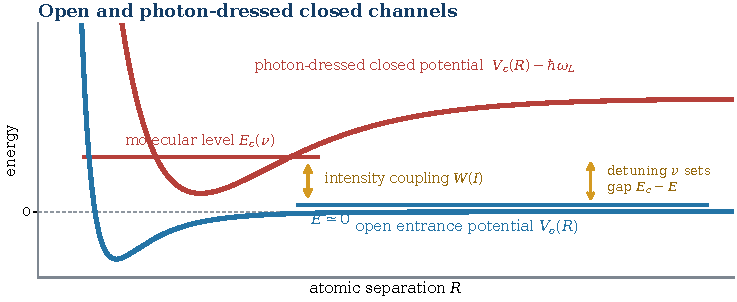
\includegraphics[width=\linewidth]{figures/figure1_ofr_schematic.pdf}
            \caption{Physical control scheme for the optical Feshbach resonance. (a) A laser couples the open-channel atom-pair continuum to a detuned excited molecular state with matrix element $W(I)$, producing the stimulated width $\Gamma(I)\propto|W|^2$; spontaneous decay at rate $\gamma$ opens the loss channel. (b) Under Eq.~\eqref{eq:ofr-dimensionless}, changing detuning $v$ moves $\ac/\ell_\star$ around a fixed-intensity locus, while changing $u=\Gamma/\gamma$ selects the locus. The elastic and inelastic quadratures are therefore linked rather than independently controllable.}
            \label{fig:ofr-schematic}
        \end{figure}

%==========================================================
\section{Model and Control Problem}\label{sec:model}
%==========================================================

    \subsection{Dimensionless variables}

        Choose a fixed positive reference time $t_\star$, independent of the
        as-yet unknown background scattering length. Its associated length is
        \begin{equation}\label{eq:reference-scales}
            t_\star=\frac{m\ell_\star^2}{\hbar},\qquad
            \ell_\star=\sqrt{\frac{\hbar t_\star}{m}},\qquad
            \tau=\frac{t}{t_\star},\qquad
            \widetilde a=\frac{a}{\ell_\star}.
        \end{equation}
        Optical frequencies are separately measured in units of $\gamma$:
        \begin{equation}\label{eq:dimensionless-controls}
            u(\tau)=\frac{\Gamma(t)}{\gamma},\qquad
            v(\tau)=\frac{\nu(t)}{\gamma}.
        \end{equation}
        The background ratio and its derived sign are
        \begin{equation}\label{eq:background-ratio}
            r_{\rm bg}=\frac{\abg}{\ell_\star}
            =\sqrt{\frac{m}{\hbar t_\star}}\,\abg,
            \qquad s=\operatorname{sgn}(r_{\rm bg}).
        \end{equation}
        Equation~\eqref{eq:ofr-dimensional} becomes the mapping implemented in the code,
        \begin{equation}\label{eq:ofr-dimensionless}
            \widetilde a_c(t)
            =|r_{\rm bg}|\left[
                s+\frac{s u(t)}{-s u(t)-v(t)-\ii/2}
            \right].
        \end{equation}
        The absolute-value prefactor is necessary because $r_{\rm bg}$ is
        stored as a signed ratio: at $u=0$, Eq.~\eqref{eq:ofr-dimensionless}
        reduces to $\widetilde a_c=r_{\rm bg}$. The value $r_{\rm bg}=0$ is
        excluded because its sign is undefined. Its nonzero magnitude and sign
        are both physical inputs and can be swept without a separate sign
        parameter.
        The admissible controls obey
        \begin{equation}\label{eq:control-bounds}
            0\leq u(t)\leq u_{\max},\qquad
            |v(t)|\leq v_{\max},
        \end{equation}
        with $u_{\max}=\Gamma_{\max}/\gamma$.

        Once a fixed $t_\star$ is selected, each candidate mass and background
        length maps to a definite $r_{\rm bg}$ through
        Eq.~\eqref{eq:background-ratio}. This retains the physical dependence
        on $m$ and $\abg$ rather than absorbing it into a species-dependent
        ruler.

        With $t=t_\star\tau$, $\eta=\ell_\star\widetilde\eta$, and $t_\star=m\ell_\star^2/\hbar$, the dimensional factor in Eq.~\eqref{eq:half-order-operator} cancels. The dimensionless history-kernel coefficient required by the short-time derivation is therefore
        \begin{equation}\label{eq:dimensionless-kernel-prefactor}
            \kappa_{\rm th}=\frac{1}{8\pi^{3/2}\sqrt{\ii}}.
        \end{equation}

        \draftnote{Derive the contact and yield units, propagate the relatively large uncertainty in $\abg$, and check that every plotted quantity is labelled either dimensionlessly or in physical units. Keep the relative-coordinate mass convention in Eq.~\eqref{eq:time-dependent-pseudopotential} consistent throughout.}

        \draftnote{The exact noninteracting start has $\eta(0)=0$. The current recurrence initializes $\eta_0=-4\pi\ac(0)$ and uses a separately coded kernel constant. Reconcile that initialization and verify the coded constant against Eq.~\eqref{eq:dimensionless-kernel-prefactor} before reporting production results.}

    \subsection{Molecular-yield objective}

        Under the sign convention in Eq.~\eqref{eq:ofr-dimensionless}, the loss--contact relation gives a non-negative product flux proportional to $-s\operatorname{Im}(1/\ac)|\eta|^2$. In the implemented dimensionless normalization, the accumulated objective is
        \begin{equation}\label{eq:molecule-objective}
            \Jmol[u,v]
            =\frac{1}{2\pi}\int_0^T
            -s\operatorname{Im}\!\left(\frac{1}{\ac(t)}\right)
            |\eta(t)|^2\,\dd t.
        \end{equation}
        This is the dimensionless, density-like quantity maximized in the current inelastic simulations. It is non-negative for either sign of $r_{\rm bg}$.

        \begin{rhoenv}[frametitle=Counting convention to resolve]
            Equation~\eqref{eq:molecule-objective} is a physical yield proxy, but the derivation must establish whether its prefactor counts depleted atoms, lost pairs, or product molecules. A positive global factor does not change the optimizing protocol, but it does change every quoted density, fraction, and molecule number. Until that factor and $g_2(0)$ are restored, report $\Jmol$ as a dimensionless objective rather than an absolute molecule count.
        \end{rhoenv}

    \subsection{Operational regularization}

        Piecewise controls can exploit the discretization by developing unrealistically sharp features. To compare physical setups without changing the effective regularization, define $\bar u=u/u_{\max}$, $\bar v=v/v_{\max}$, and $\theta=t/T$. The code therefore subtracts the normalized finite-difference penalty
        \begin{equation}\label{eq:smoothness}
            \Rsm=\frac{1}{\Delta\theta}\sum_{k=0}^{N-1}
            \left[
                \lambda_u(\bar u_{k+1}-\bar u_k)^2
                +\lambda_v(\bar v_{k+1}-\bar v_k)^2
            \right]
            ,\qquad \Delta\theta=\frac{\Delta t}{T}=\frac{1}{N}.
        \end{equation}
        Identical relative pulse shapes therefore receive identical penalties even when $T$, $u_{\max}$, or $v_{\max}$ differ. The optimizer maximizes the regularized score
        \begin{equation}\label{eq:score}
            \mathcal{S}=\Jmol-\Rsm,
        \end{equation}
        while all quoted molecular yields must report the unpenalized $\Jmol$ as well. A posteriori slew tests are applied separately to avoid interpreting the regularizer as a hardware model.

%==========================================================
\section{Numerical Methods}\label{sec:numerics}
%==========================================================

    \subsection{Time discretization and L1 history solver}

        The interval $[0,T]$ is divided into $N$ equal steps, $t_k=k\Delta t$, with controls represented at $N+1$ grid points. The L1 discretization uses the history weights
        \begin{equation}\label{eq:l1-weights}
            w_{k,j}=\sqrt{k-j}-\sqrt{k-j-1},
            \qquad 0\leq j\leq k-2.
        \end{equation}
        Defining $q=2\kappa_{\rm code}/\sqrt{\Delta t}$ for the code-level kernel prefactor and
        \begin{equation}\label{eq:l1-history}
            H_k=\sum_{j=0}^{k-2}w_{k,j}(\eta_{j+1}-\eta_j),
        \end{equation}
        the implemented recurrence has the explicit form
        \begin{equation}\label{eq:l1-update}
            \eta_k=
            \frac{-1+q(\eta_{k-1}-H_k)}
            {1/[4\pi\ac(t_k)]+q}.
        \end{equation}
        Molecular yield is then evaluated with the composite trapezoidal rule. Consistency with the continuous derivation requires the discretization, sign convention, and nondimensionalization to recover $\kappa_{\rm code}=\kappa_{\rm th}$ from Eq.~\eqref{eq:dimensionless-kernel-prefactor}.

        \draftnote{Complete a constant- or power-law benchmark that verifies the kernel coefficient and initialization independently of optimization. Then give the formal convergence order for the solution regularity, computational complexity, and measured convergence from Section~\ref{sec:validation}.}

    \subsection{Bounded physical controls}

        Unconstrained optimizer variables $x_k,y_k\in\mathbb{R}$ are mapped smoothly into the admissible laser domain:
        \begin{equation}\label{eq:bounded-map}
            u_k=u_{\max}\,\operatorname{sigmoid}(x_k),\qquad
            v_k=v_{\max}\tanh(y_k).
        \end{equation}
        This parameterization makes every iterate physical with respect to the amplitude bounds and remains differentiable for automatic differentiation. Saturation of either map can, however, reduce gradients; cap-usage diagnostics are therefore retained.

    \subsection{Gradient optimization}

        The calculation follows the logic of GRAPE: discretize the controls, differentiate the terminal performance with respect to every time slice, and update the complete pulse \cite{khaneja2005optimal}. JAX differentiates through the scattering map, Volterra scan, quadrature, and regularizer. Batched Adam updates are compiled and vectorized, with 64-bit arithmetic used for production calculations.

        The learning rate is changed in stages without resetting Adam's moment estimates. Stability is evaluated at fixed checkpoint intervals independently of those stages. For run $r$, the reported solution is the best finite iterate according to $\mathcal{S}$ when smoothing is active and according to $\Jmol$ otherwise.

    \subsection{Multi-start strategy and convergence tests}

        The current workflow combines 16 structured $u$--$v$ initializations with 24 reproducible random Fourier initializations. Selected optimized controls are perturbed with smooth, zero-mean Fourier noise to probe local robustness. Seed sensitivity is treated as a population diagnostic, not as a stopping condition for an individual run.

        At present, the internal stopping test measures motion in the raw optimizer coordinates $z\in\{x,y\}$ over a checkpoint block of $M$ steps,
        \begin{equation}\label{eq:raw-control-stability}
            \epsilon_z^{\rm raw}(k)=
            \frac{\|z_k-z_{k-M}\|_2}{\|z_k\|_2+\epsilon}.
        \end{equation}
        Because the sigmoid and $\tanh$ maps distort this distance near their bounds, final reporting should additionally use bounded, range-normalized changes
        \begin{equation}\label{eq:physical-control-stability}
            \epsilon_u=\frac{\|u_k-u_{k-M}\|_2}{\sqrt{N+1}\,u_{\max}},\qquad
            \epsilon_v=\frac{\|v_k-v_{k-M}\|_2}{2\sqrt{N+1}\,v_{\max}}.
        \end{equation}
        A run is accepted only after the regularized score and every active control pass their tolerances for the required number of consecutive checkpoints. The score test, raw-coordinate stopping test, and bounded-control diagnostic must be labelled separately in figures and archived data.

        \begin{table}[H]
            \caption{Baseline $N=100$ numerical protocol encoded in the current calibration workflow. Confirm or replace these entries when production settings are frozen.}
            \label{tab:numerical-protocol}
            \setlength{\tabcolsep}{3pt}
            \begin{tabular}{>{\raggedright\arraybackslash}p{0.43\columnwidth}>{\raggedright\arraybackslash}p{0.42\columnwidth}}
                \toprule
                \textbf{Quantity} & \textbf{Current value} \\
                \midrule
                Grid intervals $N$ & $100$ \\
                Initial learning rate & $10^{-2}$ \\
                Stage schedule & $(5000,1)$, $(5000,0.5)$, $(7500,0.5)$, $(7500,0.5)$ \\
                Stability interval & $500$ steps \\
                Consecutive passes & $3$ \\
                Score tolerance & $10^{-5}$ \\
                Raw-control tolerances & $10^{-3}$ for $x$ and $y$ \\
                Initializations & $16$ structured $+24$ Fourier \\
                Smoothness scan & $17$ log-spaced points over $10^{-4}$--$1$ \\
                Shared slew parameter & $0.05$ \\
                Arithmetic & JAX float64 \\
                \bottomrule
            \end{tabular}
            \tabletext{Learning-rate multipliers compound between stages. The smoothness selection currently weights valid-run yield by $0.7$ and roughness by $0.3$.}
        \end{table}

    \subsection{Calibration sequence and reproducibility}

        The production methodology fixes hyperparameters in a prescribed order:
        \begin{enumerate}
            \item select the learning-rate schedule at $N=100$;
            \item calibrate the shared smoothness against yield and slew validity;
            \item sweep the initial intensity cap using those frozen settings; and
            \item perform the final $u_{\max}$ sweep and robustness checks.
        \end{enumerate}
        Numerical data, metadata, and figures are stored separately so that plots can be recreated without rerunning the optimizer.

        \begin{figure}[H]
            \centering
            \figureplaceholder[39mm]{Show the dependency graph: physics configuration $\rightarrow$ batched controls $\rightarrow$ scattering map $\rightarrow$ Volterra solver $\rightarrow$ objective/penalty $\rightarrow$ autodiff/Adam $\rightarrow$ CSV and figures.}
            \caption{Computational workflow and artifact flow. Annotate the source-labelled directories used for configurations, results, figures, and logs.}
            \label{fig:workflow}
        \end{figure}

%==========================================================
\section{Verification and Validation}\label{sec:validation}
%==========================================================

    \subsection{Analytical checks of the scattering map}

        Equation~\eqref{eq:ofr-dimensionless} should be checked in three limits before optimization: $u\rightarrow0$ gives $\ac\rightarrow\abg$; large $|v|$ suppresses the optical shift and loss; and the near-resonant response reproduces the expected dispersive real part and absorptive imaginary part. These checks also establish the sign conventions for $v$ and $\operatorname{Im}\ac$.

        \begin{table}[H]
            \caption{Minimum validation matrix. Replace the final column with measured errors and pass criteria.}
            \label{tab:validation-matrix}
            \setlength{\tabcolsep}{3pt}
            \begin{tabular}{>{\raggedright\arraybackslash}p{0.30\columnwidth}>{\raggedright\arraybackslash}p{0.34\columnwidth}>{\raggedright\arraybackslash}p{0.23\columnwidth}}
                \toprule
                \textbf{Test} & \textbf{Expected behaviour} & \textbf{Result} \\
                \midrule
                No laser & $\ac/\abg\to1$ & [insert] \\
                Far detuned & optical term $\to0$ & [insert] \\
                Complex sign & $\operatorname{Im}\ac<0$ & [insert] \\
                Constant $a_s$ & known/reference $\eta(t)$ & [insert] \\
                Square-root ramp & universal onset law & [insert] \\
                Grid refinement & convergent $\Jmol$ and pulse & [insert] \\
                Autodiff gradient & finite-difference agreement & [insert] \\
                \bottomrule
            \end{tabular}
        \end{table}

    \subsection{Volterra solver and quadrature convergence}

        Optimization stability at fixed $N$ is not evidence of time-grid convergence. For a sequence such as $N=100,200,400,800,1000$, define the relative yield difference
        \begin{equation}\label{eq:grid-error}
            \epsilon_N=
            \frac{|\Jmol^{(N)}-\Jmol^{(N_{\rm fine})}|}
            {\max(|\Jmol^{(N_{\rm fine})}|,10^{-12})}.
        \end{equation}
        If no analytic reference is available, the difference between the two finest grids is an error estimate, not a rigorous bound. Report the error in $\eta(t)$ where a reference is available and whether qualitative control features persist. Because optimization can exploit grid-specific structure, use both routes: evaluate one fixed interpolated pulse on every grid, and independently reoptimize to comparable convergence at every $N$.

        \begin{figure}[H]
            \centering
            \figureplaceholder[48mm]{Panel (a): real and imaginary parts of $\eta(t)$ for several $N$. Panel (b): relative yield error versus $\Delta t$ on log axes with a fitted slope. Panel (c): optimized controls after interpolation to a common grid.}
            \caption{Validation and grid-convergence tests for the L1 Volterra solver and optimized objective. State the reference solution and error norm in the caption.}
            \label{fig:solver-validation}
        \end{figure}

    \subsection{Gradient and baseline checks}

        On a reduced grid, compare automatic derivatives of $\mathcal{S}$ with centered finite differences for randomly selected control components. Then reproduce the real-scattering-length or unconstrained baseline associated with the universal onset problem before introducing the physical OFR mapping.

        \draftnote{Give numerical tolerances, hardware, software versions, and the commit identifier. A statement such as ``the curves look similar'' is not a validation criterion; quote norms and relative errors.}

%==========================================================
\section{Results}\label{sec:results}
%==========================================================

    \subsection{Learning-rate and convergence calibration}

        Present the evidence used to select the staged Adam schedule. Separate the unpenalized physical objective $\Jmol$, smoothness penalty $\Rsm$, and regularized score $\mathcal{S}$, and show the checkpoint-based convergence criteria for the best and median initializations.

        \begin{rhoenv}[frametitle=Provisional optimizer observation]
            The project log records an exploratory schedule with one $(5000,1)$ stage followed by nine $(5000,0.5)$ stages. From an initial rate $10^{-2}$, the nine cumulative halvings give a final rate $1.95\times10^{-5}$ without resetting Adam's moments. Under the metric then in use, the objective change reached approximately $10^{-10}$ while the two control changes remained just above $10^{-3}$. Most starts approached similar controls, but one reached zero yield; milder annealing retained a wider family of controls. These observations must be reproduced from archived run data before being promoted to quantitative results. They suggest a shallow or poorly conditioned optimum, not an exactly flat objective.
        \end{rhoenv}

        Use the fully annealed ensemble for the primary yield estimate once reproduced; use milder schedules only to diagnose the landscape. Numerical precision in the reported yield is limited by the grid-convergence study, even when optimizer stability is much smaller.

        \begin{figure*}[t]
            \centering
            \figureplaceholder[48mm]{Recommended panels: $\Jmol$, $\Rsm$, and $\mathcal{S}$ histories with learning-rate boundaries; score stability; bounded $\epsilon_u$ and $\epsilon_v$ from Eq.~\eqref{eq:physical-control-stability}; final-yield distribution including failures. Overlay all converged controls faintly, with the median or best protocol emphasized.}
            \caption{Learning-rate calibration and convergence diagnostics at $N=100$. Vertical markers should identify stage changes and horizontal markers the stopping tolerances. Report $n_{\rm success}/40$, define failure before inspecting outcomes, and display rather than silently remove any zero-yield run.}
            \label{fig:convergence}
        \end{figure*}

        \draftnote{Archive and reproduce the ten-stage observation, then state which schedule was selected and why. Diagnose any zero-yield start by checking $u\simeq0$, saturation of raw variables, gradient norms, and non-finite values; unless it is shown to be a valid stationary solution, classify it as an optimization failure.}

    \subsection{Shallow-landscape diagnosis}

        Similar values of $\Jmol$ need not imply identical controls. Let $(u^\star,v^\star)$ be the best converged protocol and define, for run $i$,
        \begin{align}\label{eq:landscape-distance}
            d_u^{(i)}&=\frac{\|u^{(i)}-u^\star\|_2}{\sqrt{N+1}\,u_{\max}}, &
            d_v^{(i)}&=\frac{\|v^{(i)}-v^\star\|_2}{2\sqrt{N+1}\,v_{\max}},\nonumber\\
            d_{uv}^{(i)}&=\sqrt{(d_u^{(i)})^2+(d_v^{(i)})^2}, &
            \Delta J^{(i)}&=\frac{\Jmol^\star-\Jmol^{(i)}}{|\Jmol^\star|}.
        \end{align}
        A broad range of $d_{uv}$ at small $\Delta J$ supports a shelf of nearly equivalent solutions. Plot both $\Jmol$ and $\mathcal{S}$: flat $\Jmol$ but curved $\mathcal{S}$ means the regularizer selects a smooth representative, whereas flatness in both gives stronger evidence of a shallow physical landscape.

        Confirm this with no-reoptimization line scans in raw optimizer space, $z(\lambda)=(1-\lambda)z^\star+\lambda z^{(i)}$. Compare not only the controls but the induced $\ac(t)$, $|\eta(t)|^2$, and flux $\operatorname{Im}(1/\ac)|\eta|^2$: visibly different laser waveforms may be physically equivalent after the nonlinear scattering map and history dynamics.

    \subsection{Smoothness and slew calibration}

        The shared coefficient $\lambda_u=\lambda_v=\lambda$ is scanned logarithmically. The choice must balance physical yield against roughness while satisfying separate normalized slew limits for both controls. Report all run-level points, not only medians, so that failure fractions and outliers remain visible.

        \begin{figure*}[t]
            \centering
            \figureplaceholder[52mm]{Combine the generated calibration figures: (a) normalized $u$ slew versus $\lambda$; (b) normalized $v$ slew versus $\lambda$; (c) valid-run median yield and roughness or weighted selection score. Mark the selected $\lambda$.}
            \caption{Smoothness calibration under the configured slew constraints. Define the slew metric, valid-run criterion, and selection rule in the caption.}
            \label{fig:smoothness-calibration}
        \end{figure*}

        \draftnote{Report the selected $\lambda$, valid-run fraction, loss in unpenalized yield relative to weak regularization, and sensitivity of the choice to the 0.7/0.3 selection weighting.}

    \subsection{Optimized laser-constrained protocol}

        For one representative cap, show how the optimized physical controls generate the complex scattering length, pair amplitude, instantaneous molecular flux, and cumulative yield. This is the key figure for explaining the mechanism rather than only the performance.

        \begin{figure*}[t]
            \centering
            \figureplaceholder[62mm]{Recommended panels: (a) $u(t)$ with $u_{\max}$; (b) $v(t)$ with detuning bounds; (c) trajectory of $\ac/\abg$ in the complex plane; (d) $|\eta(t)|^2$; (e) instantaneous $\operatorname{Im}(1/\ac)|\eta|^2/(2\pi)$; (f) cumulative $\Jmol(t)$.}
            \caption{Representative optimized protocol and its physical response. Use a common normalized time axis, mark cap-active intervals, and identify which historical features build contact before molecular conversion.}
            \label{fig:optimal-protocol}
        \end{figure*}

        \draftnote{Explain the pulse chronologically. Distinguish observations visible in the data from physical interpretations such as contact preparation, conversion, or quantum-Zeno-like suppression.}

    \subsection{Yield versus available laser power}

        The master result is obtained by sweeping $u_{\max}=\Gamma_{\max}/\gamma$ over approximately three decades while holding the validated numerical methodology fixed. Both best and median multi-start yields should be shown. The normalized cap usage
        \begin{equation}\label{eq:cap-usage}
            r_u=\max_k\frac{u_k}{u_{\max}}
        \end{equation}
        distinguishes power-limited solutions from those that leave additional intensity unused.

        \begin{figure*}[t]
            \centering
            \figureplaceholder[58mm]{Panel (a): optimized $\Jmol$ versus $u_{\max}$ on a logarithmic cap axis, with best, median, and run spread. Add the unconstrained/universal benchmark where justified. Panel (b): median and maximum $r_u$. Shade tight-cap, crossover, and saturation regimes.}
            \caption{Optimized molecular yield as a function of the available optical coupling. Define the statistical summary, cap-binding threshold, uncertainty band, and criterion used to identify saturation.}
            \label{fig:cap-sweep}
        \end{figure*}

        \begin{table}[H]
            \caption{Quantitative comparison of the regimes in \figref{fig:cap-sweep}.}
            \label{tab:cap-regimes}
            \setlength{\tabcolsep}{3pt}
            \begin{tabular}{>{\raggedright\arraybackslash}p{0.27\columnwidth}>{\raggedright\arraybackslash}p{0.25\columnwidth}>{\raggedright\arraybackslash}p{0.34\columnwidth}}
                \toprule
                \textbf{Regime} & \textbf{$u_{\max}$ range} & \textbf{Observed behaviour} \\
                \midrule
                Tight cap & [insert] & [yield scaling and $r_u$] \\
                Crossover & [insert] & [pulse/mechanism change] \\
                Saturation & [insert] & [plateau criterion] \\
                \bottomrule
            \end{tabular}
        \end{table}

        \draftnote{Quote the fitted low-cap scaling if supported, the crossover cap, the plateau yield, and the incremental gain from the largest tested cap. Do not infer a true asymptote from too narrow a sweep.}

    \subsection{Robustness and uncertainty}

        Robustness should cover at least initialization seed, grid resolution, convergence tolerance, smoothness choice, and modest perturbations to the final controls. Treat zero or non-finite yield as a reported failure category rather than filtering it from the seed statistics. Where experimental parameters are uncertain, repeat the final protocol for representative variations in $\gamma$, intensity calibration, and detuning offset.

        \begin{figure}[H]
            \centering
            \figureplaceholder[47mm]{Summarize seed spread and robustness: final-yield distribution with failures; $\Delta J$ versus $d_{uv}$; raw-space line scans of $\Jmol$ and $\mathcal{S}$; yield after smooth Fourier perturbations; and relative changes under grid or parameter variations.}
            \caption{Numerical, landscape, and control robustness of the optimized yield. Give the total and successful run counts, define every perturbation distribution, and distinguish optimizer spread from discretization error.}
            \label{fig:robustness}
        \end{figure}

%==========================================================
\section{Experimental Translation}\label{sec:experiment}
%==========================================================

    \subsection{Fixed representative: bosonic strontium-88}

        The physical reference is an $^{88}\mathrm{Sr}$ condensate in the $^1S_0+{}^1S_0$ entrance channel, optically coupled near the $^1S_0+{}^3P_1$ molecular asymptote. The atomic intercombination line is near $689\,\mathrm{nm}$; its measured $^{88}\mathrm{Sr}$ frequency is $434\,829\,121\,311(10)\,\mathrm{kHz}$ \cite{ferrari2003precision}. The condensate experiment used the second-least-bound excited molecular level, with binding energy $h\times24\,\mathrm{MHz}$ below this asymptote \cite{yan2013controlling}.

        The measured intensity calibration is naturally expressed through the optical length $\ell_{\rm opt}$ rather than a universal constant $\xi$:
        \begin{equation}\label{eq:sr-intensity-calibration}
            \ell_{\rm opt}=\beta I,\qquad
            \Gamma_{\rm stim}=2k_r\ell_{\rm opt}\Gamma_{\rm mol},\qquad
            \beta=2.2\times10^4\frac{a_0}{\mathrm{W\,cm^{-2}}},
        \end{equation}
        where $k_r$ is the relative collision wave number and $\Gamma_{\rm mol}=2\pi\times15\,\mathrm{kHz}$ \cite{yan2013controlling}. If the model quantities are identified as $\Gamma=\Gamma_{\rm stim}$, $\gamma=\Gamma_{\rm mol}$, and $\nu=\Delta$, then
        \begin{equation}\label{eq:intensity-conversion}
            I_{\max}=\frac{u_{\max}}{2k_r\beta},\qquad
            \frac{\Delta(t)}{2\pi}=\left(15\,\mathrm{kHz}\right)v(t).
        \end{equation}
        Thus an intensity cap cannot be assigned until $k_r$ is fixed consistently from the simulated gas. By contrast, the current $v_{\max}=50$ maps directly to $|\Delta|/2\pi=0.75\,\mathrm{MHz}$, within the experimentally explored range.

        \begin{table*}[t]
            \caption{Fixed $^{88}\mathrm{Sr}$ reference parameters. ``Derived'' values use the central reported quantities and are not additional measurements.}
            \label{tab:experimental-parameters}
            \setlength{\tabcolsep}{5pt}
            \begin{tabular}{>{\raggedright\arraybackslash}p{0.20\textwidth}>{\raggedright\arraybackslash}p{0.54\textwidth}>{\raggedright\arraybackslash}p{0.16\textwidth}}
                \toprule
                \textbf{Parameter} & \textbf{Value} & \textbf{Source} \\
                \midrule
                Isotope and channel & Bosonic $^{88}\mathrm{Sr}$; $^1S_0+{}^1S_0\rightarrow{}^1S_0+{}^3P_1$ & \cite{blatt2011measurement,yan2013controlling} \\
                Atomic line & $689\,\mathrm{nm}$; $434\,829\,121\,311(10)\,\mathrm{kHz}$ & \cite{ferrari2003precision} \\
                Background length & $\abg=-1.4(6)a_0$; the condensate paper uses the rounded value $-2a_0$ & \cite{blatt2011measurement,yan2013controlling} \\
                Molecular reference & Second-least-bound level at $-24\,\mathrm{MHz}$; $\Gamma_{\rm mol}/2\pi=15\,\mathrm{kHz}$ & \cite{yan2013controlling} \\
                Optical coupling & $\ell_{\rm opt}/I=2.2\times10^4a_0/(\mathrm{W\,cm^{-2}})$; at $0.057\,\mathrm{W\,cm^{-2}}$, $\ell_{\rm opt}=1.25\times10^3a_0$ & \cite{yan2013controlling}; derived \\
                Demonstrated controls & $|\Delta|/2\pi$ up to $10\,\mathrm{MHz}$, or $|\Delta|/\Gamma_{\rm mol}\simeq667$; typical $a=20a_0$ at $+1\,\mathrm{MHz}$; changes up to $a_{\rm opt}/\abg=\pm10$ & \cite{yan2013controlling} \\
                Condensate & $N_0\simeq7000$, peak density $n_0=1\times10^{15}\,\mathrm{cm^{-3}}$, initial size $\sigma_0=0.8\,\mu\mathrm{m}$, trap mean frequency $2\pi\times(60\pm5)\,\mathrm{Hz}$ & \cite{yan2013controlling} \\
                Laser and timing & Waist $725\,\mu\mathrm{m}$; example intensity $0.057\,\mathrm{W\,cm^{-2}}$; $1.2$- and $4$-ms exposures. The intensity corresponds to $0.47\,\mathrm{mW}$ for an on-axis Gaussian convention & \cite{yan2013controlling}; derived \\
                Loss scale & $K_{\rm in}\sim10^{-12}\,\mathrm{cm^3\,s^{-1}}$, millisecond sample lifetimes, fitted enhancement $\eta_{\rm loss}=19.5$ & \cite{yan2013controlling} \\
                \bottomrule
            \end{tabular}
        \end{table*}

    \subsection{Experimentalist's recipe}

        Use $I=0.057\,\mathrm{W\,cm^{-2}}$, waist $725\,\mu\mathrm{m}$, and detunings of order $1\,\mathrm{MHz}$ as a literature-anchored comparison point, not yet as the optimized recommendation. The quoted beam corresponds to approximately $0.47\,\mathrm{mW}$ if $I$ is the peak intensity of a Gaussian beam. Once the fixed reference time $t_\star$ has been selected, the reported $1.2$- and $4$-ms exposures must be converted using $\tau=t/t_\star$; they cannot be represented by silently setting the solver's $T=1$ equal to one millisecond.

        The experimental isolated-resonance model contains the fitted loss enhancement $\eta_{\rm loss}=19.5$ and a detuning-dependent background loss not present in Eq.~\eqref{eq:ofr-dimensional} \cite{yan2013controlling}. The subscript distinguishes this empirical loss parameter from the pair amplitude $\eta(t)$ in Eq.~\eqref{eq:contact-eta}. The $^{88}\mathrm{Sr}$ prescription is therefore conditional on first verifying the mapping between the measured model and the implemented $\ac(u,v)$, especially the roles of $\Gamma_{\rm stim}$, $\Gamma_{\rm mol}$, and the phenomenological loss terms.

        \begin{figure*}[t]
            \centering
            \figureplaceholder[54mm]{Primary axis: predicted $^{88}\mathrm{Sr}$ molecular yield/fraction versus peak $689$-nm intensity, with a power axis for $w=725\,\mu\mathrm{m}$. Mark $0.057\,\mathrm{W\,cm^{-2}}$ as the literature comparison and the optimized operating point separately. Inset: intensity and detuning waveforms in ms and MHz relative to the $-24$-MHz PA level.}
            \caption{Experimental prescription for $^{88}\mathrm{Sr}$. Propagate uncertainty in $\abg$, $\ell_{\rm opt}/I$, density, and collision momentum; state whether the prediction is a dimensionless objective, density, fraction, or absolute molecule number.}
            \label{fig:experimental-recipe}
        \end{figure*}

        \draftnote{Calculate $k_r$ for the final cloud model, convert every optimized $u(t)$ through Eq.~\eqref{eq:intensity-conversion}, and compare the resulting peak power, modulation bandwidth, and duration with Table~\ref{tab:experimental-parameters}. Re-run the dynamics with the measured enhanced and background loss before claiming a quantitative $^{88}\mathrm{Sr}$ molecule yield.}

%==========================================================
\section{Discussion}\label{sec:discussion}
%==========================================================

    \subsection{Physical interpretation}

        \draftnote{Explain why the optimal history outperforms simple constant, linear, square-root, or bang--bang trial protocols. Relate the protocol to the competition between building contact and converting correlated pairs into products. If invoking a quantum-Zeno mechanism, show the diagnostic that supports it.}

        Compare the cap sweep with the scale-invariant real-$a_s$ onset of Ref.~\cite{qi2021maximum}. Make explicit which aspects remain universal and which are introduced by the optical map, finite decay rate, detuning bound, and control regularization.

    \subsection{Comparison with baseline protocols}

        \begin{table}[H]
            \caption{Performance comparison at a common duration and cap.}
            \label{tab:protocol-comparison}
            \setlength{\tabcolsep}{3pt}
            \begin{tabular}{>{\raggedright\arraybackslash}p{0.35\columnwidth}>{\raggedright\arraybackslash}p{0.20\columnwidth}>{\raggedright\arraybackslash}p{0.28\columnwidth}}
                \toprule
                \textbf{Protocol} & \textbf{$\Jmol$} & \textbf{Relative to optimum} \\
                \midrule
                Best constant controls & [insert] & [insert] \\
                Simple ramp & [insert] & [insert] \\
                Square-root-inspired & [insert] & [insert] \\
                Unconstrained baseline & [insert] & [insert] \\
                Optimized OFR controls & [insert] & $1$ \\
                \bottomrule
            \end{tabular}
        \end{table}

    \subsection{Limitations}

        The final report should assess at least the following limitations:
        \begin{itemize}
            \item validity of the universal short-time, zero-range, and dilute-gas approximations;
            \item neglect of depletion, many-body feedback, trapping inhomogeneity, and additional loss channels;
            \item accuracy and convention dependence of the two-channel OFR map;
            \item numerical bias from finite $N$, smoothness selection, bounded parameterization, and local optimization;
            \item distinction between the finite-difference slew diagnostic and a measured laser transfer function;
            \item collision-momentum dependence in translating $\Gamma$ to $689$-nm intensity for $^{88}\mathrm{Sr}$; and
            \item omission of the measured $\eta_{\rm loss}=19.5$ enhancement and far-wing background loss from the implemented optical map.
        \end{itemize}

        \draftnote{For each material limitation, state the likely direction of bias and one concrete test or future extension.}

    \subsection{Mathematical and computational extensions}

        After the baseline calculation is validated, the Hessian spectrum of $\mathcal{S}$ can quantify poorly constrained control directions more directly than endpoint scatter alone. Hessian-vector products or a reduced-basis eigenspectrum are preferable to forming the full dense Hessian. Quasi-Newton polishing can then be compared fairly with the long Adam anneal. A robust-control extension should maximize an ensemble average, or a risk-sensitive alternative, over calibrated Gaussian laser-amplitude and detuning noise. Physics-informed neural networks remain a possible surrogate for the nonlocal dynamics, but only after their accuracy and cost are benchmarked against the L1 solver.

%==========================================================
\section{Conclusion}\label{sec:conclusion}
%==========================================================

    \draftnote{Write this section only after the figures are final. In one compact paragraph: answer the central question; quote the optimal/plateau yield and crossover cap; state the representative laboratory requirement; summarize robustness; and give the most important limitation. Follow with 2--3 specific next steps.}

    The completed conclusion should distinguish the scientific result---how a physical laser constraint shapes the optimal molecular yield---from the computational deliverable of a validated, reproducible JAX workflow.

%==========================================================
\section*{Author Contributions}
\addcontentsline{toc}{section}{Author Contributions}
%==========================================================

    \draftnote{Use the CRediT taxonomy if appropriate. State the student's work and the supervisor's roles in conceptualization, methodology, software, analysis, supervision, and writing.}

%==========================================================
\section*{Acknowledgements}
\addcontentsline{toc}{section}{Acknowledgements}
%==========================================================

    \draftnote{Acknowledge the supervisor, collaborators, CUHK programme support, computing resources, and any funding.}

%==========================================================
\section*{Data and Code Availability}
\addcontentsline{toc}{section}{Data and Code Availability}
%==========================================================

    The reusable package under \texttt{src/optical\_feshbach\_control/} separates calculations, analysis, plotting, and artifact I/O. Versioned run settings belong in \texttt{configs/}; numerical artifacts in \texttt{results/}; regenerated graphics in \texttt{figures/}; and queue logs in \texttt{logs/}. The $N=100$ calibration notebooks and non-interactive smoothness workflow record the ordered methodology used in this report.

    \draftnote{Add the repository URL or archive DOI, exact commit hash, environment file, commands needed to reproduce every final figure, and any access restrictions.}

%==========================================================
\appendix
\section{Nondimensionalization and Conventions}\label{app:nondimensionalization}
%==========================================================

    \draftnote{Extend the dimensional audit above to the contact and molecular-yield normalizations. Track the sign of the imaginary scattering length and all factors of $2$, $\pi$, $\hbar$, and mass, then verify the ledger against the implementation.}

    \begin{table}[H]
        \caption{Symbol and unit ledger for the final derivation.}
        \label{tab:symbol-ledger}
        \setlength{\tabcolsep}{3pt}
        \begin{tabular}{>{\raggedright\arraybackslash}p{0.20\columnwidth}>{\raggedright\arraybackslash}p{0.41\columnwidth}>{\raggedright\arraybackslash}p{0.23\columnwidth}}
            \toprule
            \textbf{Symbol} & \textbf{Meaning} & \textbf{Unit/scale} \\
            \midrule
            $\abg$ & background scattering length & $-1.4(6)a_0$ \\
            $\ac$ & complex scattering length & length; scale $|\abg|$ \\
            $\gamma$ & molecular decay rate & $2\pi\times15\,\mathrm{kHz}$ \\
            $\Gamma$ & stimulated optical width & $2k_r\ell_{\rm opt}\Gamma_{\rm mol}$ \\
            $\nu$ & detuning from $-24$-MHz PA level & angular frequency \\
            $\eta(t)$ & short-range pair amplitude & length; scale $|\abg|$ \\
            $\mathcal{C}$ & Tan-contact density & inverse length$^4$ \\
            $\Jmol$ & current yield objective & dimensionless; prefactor unresolved \\
            \bottomrule
        \end{tabular}
    \end{table}

%==========================================================
\section{Discrete Solver Derivation}\label{app:l1-derivation}
%==========================================================

    \draftnote{Derive the L1 weights and recurrence in Eqs.~\eqref{eq:l1-weights}--\eqref{eq:l1-update}. State how the endpoint singularity is handled, why the newest increment enters the denominator, and the memory/time complexity of the scan.}

%==========================================================
\section{Additional Optimization Diagnostics}\label{app:diagnostics}
%==========================================================

    \draftnote{Place full per-seed convergence plots, zero-yield diagnostics, raw- versus bounded-control stability, alternative schedules, raw-space line scans, smoothness sensitivity, and higher-resolution cap-sweep tables here. Keep only decision-relevant summaries in the main text.}

%==========================================================
\section{Reproduction Checklist}\label{app:reproduction}
%==========================================================

    \begin{enumerate}
        \item Record the repository commit and Python environment.
        \item Freeze the learning-rate, smoothness, convergence, and initialization settings.
        \item Save run-level CSV/JSON data before plotting.
        \item Label every result by grid, seed, cap, and configuration.
        \item Regenerate report figures from saved numerical artifacts.
        \item Confirm that all reported headline values can be read from an archived table.
    \end{enumerate}

% The following temporary analysis used |a_bg| as the reference length and is
% retained in the source history only. It is superseded by the fixed-time
% nondimensionalization below and intentionally omitted from the report.
\iffalse
%==========================================================
\section{Superseded Note: Unknown Background Scattering Length and a Generic Reference Scale}
\label{app:temporary-generic-length-scale}
%==========================================================

    \textbf{Status of this note.} This section is a temporary explanation of the
    nondimensionalization issue and should be reconciled with
    Sec.~\ref{sec:model} before the final report is submitted.  Its main point is
    that a reference length is a freely chosen positive unit, whereas the sign
    and magnitude of the background scattering length are physical inputs.  A
    change of units cannot determine or remove those physical inputs.

    \subsection{What can be chosen before the atomic species is known?}

        Start from the dimensional Volterra equation
        \begin{equation}\label{eq:temporary-dimensional-volterra}
            \left[
                \mathcal L_{1/2}^{(t)}
                +\frac{1}{4\pi a_s(t)}
            \right]\eta(t)=-1.
        \end{equation}
        Choose an arbitrary \emph{positive} reference length $L_0>0$ and define
        \begin{equation}\label{eq:temporary-generic-scales}
            t_0=\frac{mL_0^2}{\hbar},\qquad
            \tau=\frac{t}{t_0},\qquad
            \widetilde a_s=\frac{a_s}{L_0},\qquad
            \widetilde\eta=\frac{\eta}{L_0}.
        \end{equation}
        The factor $t_0=mL_0^2/\hbar$ makes the coefficient of the
        half-order operator dimensionless.  Equation~\eqref{eq:temporary-dimensional-volterra}
        then has the universal form
        \begin{equation}\label{eq:temporary-generic-volterra}
            \left[
                \widetilde{\mathcal L}_{1/2}^{(\tau)}
                +\frac{1}{4\pi\widetilde a_s(\tau)}
            \right]\widetilde\eta(\tau)=-1.
        \end{equation}
        Nothing in this step requires prior knowledge of $a_{\rm bg}$.  The
        choice of $L_0$ fixes the ruler and clock, but it does not specify the
        interaction measured with that ruler.

    \subsection{Where the unknown background scattering length enters}

        For the corrected optical map, define the resonant contribution
        \begin{equation}\label{eq:temporary-optical-factor}
            R(u,v)=\frac{u}{-v-u+\ii/2}.
        \end{equation}
        The stimulated coupling contains an inverse factor of
        $a_{\rm bg}$.  Its sign therefore cancels the background sign in the
        resonant correction, giving
        \begin{equation}
            a_s=a_{\rm bg}+|a_{\rm bg}|R(u,v).
        \end{equation}
        A generic nondimensionalization contains both the signed background
        ratio and its positive magnitude,
        \begin{equation}\label{eq:temporary-background-ratio}
            b=\frac{a_{\rm bg}}{L_0},
            \qquad r=\frac{|a_{\rm bg}|}{L_0}=|b|,
            \qquad \widetilde a_s=b+rR(u,v).
        \end{equation}
        Substitution into Eq.~\eqref{eq:temporary-generic-volterra} gives
        \begin{equation}\label{eq:temporary-volterra-with-background}
            \left[
                \widetilde{\mathcal L}_{1/2}^{(\tau)}
                +\frac{1}{4\pi[b+rR(u,v)]}
            \right]\widetilde\eta(\tau)=-1.
        \end{equation}
        Thus $b$ is an input to the dynamics.  Its sign cannot be inferred by
        nondimensionalization, and changing its sign is not a constant
        conversion applied after the calculation.  It changes the complex
        scattering-length history seen by the Volterra equation and can change
        both $\widetilde\eta$ and the optimal controls.  A genuinely
        species-independent calculation must consequently retain $b$ as a
        parameter or sweep over candidate positive and negative values.

        This is no different in principle from not knowing a mass, linewidth,
        or density before choosing an atom: the equations can be written with
        symbolic dimensionless parameters, but a species-specific numerical
        prediction requires those parameters to be supplied eventually.

    \subsection{The sign when using the background magnitude as reference}

        If one chooses
        \begin{equation}
            L_0=|a_{\rm bg}|,
            \qquad s=\operatorname{sgn}(a_{\rm bg}),
        \end{equation}
        then $r=1$, $b=s$, and the dimensionless scattering length is
        \begin{equation}\label{eq:temporary-signed-background}
            \widetilde a_s
            =\frac{a_s}{|a_{\rm bg}|}
            =s+\frac{u}{-v-u+\ii/2}.
        \end{equation}
        The dimensionless Volterra equation becomes
        \begin{equation}\label{eq:temporary-signed-ratio-volterra}
            \left[
                \widetilde{\mathcal L}_{1/2}^{(\tau)}
                +\frac{1}{4\pi[s+R(u,v)]}
            \right]\widetilde\eta(\tau)=-1.
        \end{equation}
        The sign therefore remains in the Volterra dynamics, but it does not
        reverse the lossy optical term.  Indeed,
        \begin{equation}
            \operatorname{Im}R(u,v)
            =-\frac{u/2}{(u+v)^2+1/4}\leq0
        \end{equation}
        for both values of $s$.  Hence
        $\operatorname{Im}(1/\widetilde a_s)\geq0$, so the implemented
        molecular objective remains non-negative for positive and negative
        background scattering lengths.  Changing $s$ can nevertheless change
        $\widetilde\eta$ and the optimal controls through the real background
        offset.

    \subsection{Does changing the reference length change the optimization?}

        Merely changing $L_0$ does not change a fixed physical problem when
        every dimensionless quantity is transformed consistently.  For a
        physical duration $t_{\rm f}$, the solver horizon must be
        \begin{equation}\label{eq:temporary-duration-conversion}
            T=\frac{t_{\rm f}}{t_0}
             =\frac{\hbar t_{\rm f}}{mL_0^2}.
        \end{equation}
        At the same time, the solver must receive
        $b=a_{\rm bg}/L_0$ and the correspondingly scaled scattering length and
        pair amplitude.  Two calculations using different $L_0$ but describing
        the same $t_{\rm f}$, $a_{\rm bg}$, and laser history should then be
        related by a change of variables.

        By contrast, changing $L_0$ while retaining $T=1$ changes the physical
        duration to $t_{\rm f}=mL_0^2/\hbar$.  Likewise, replacing an unknown
        $b$ by $+1$ chooses a positive-background model.  These changes affect
        the optimization itself and are not post-processing conversions.  In
        the present numerical implementation, $T$ enters the time step, the
        history kernel, the objective integral, and the smoothness penalty, so
        it cannot generally be altered only when plotting the final result.

    \subsection{A practical species-independent workflow}

        A clean workflow is:
        \begin{enumerate}
            \item Choose and document a positive reference length $L_0$.  It
            may be a fixed nominal length used across species or a physically
            motivated range scale.  It must not be a signed quantity.
            \item Keep $b=a_{\rm bg}/L_0$ as an explicit signed model
            parameter.  If the target species is not yet chosen, sample a
            physically motivated range of both signs rather than silently
            setting $b=1$.
            \item Specify or sweep the dimensionless horizon $T$.  Once an atom
            and a desired laboratory duration are selected, use
            Eq.~\eqref{eq:temporary-duration-conversion} to determine its
            appropriate value.
            \item Optimize using
            $\widetilde a_s=b+|b|R(u,v)$ in the Volterra recurrence and in the
            molecular objective.  With $L_0=|a_{\rm bg}|$, this reduces to
            $\widetilde a_s=s+R(u,v)$.  The recurrence algorithm does not need
            to be re-derived for each atom; only its dimensionless inputs
            change.
            \item After selecting a species, insert its mass, signed
            $a_{\rm bg}$, linewidth, density, and control calibration.  Check
            the zero-range and short-many-body-time validity window before
            interpreting the result as a laboratory protocol.
        \end{enumerate}

        In code, the scale choice $L_0=|a_{\rm bg}|$ is represented by the
        searchable scalar parameter \texttt{scattering\_sign}$=s$.  The
        implementation uses $s+R(u,v)$ and validates $s\in\{-1,+1\}$.

    \paragraph{Direct answer.}
        It was not incorrect to use the magnitude of the background scattering
        length as a convenient scale after a species had been selected.  It was
        incorrect to expect that choice to make an unknown signed
        $a_{\rm bg}$ universally equal to $+1$.  Before the species is known,
        either retain $b=a_{\rm bg}/L_0$ symbolically or include it in the
        parameter sweep.  After the species is known, choosing
        $L_0=|a_{\rm bg}|$ reduces $b$ to its sign.  That sign is added to the
        resonant term in the scattering map and must still be supplied to the
        $\eta$ calculation.

\fi

%==========================================================
\section{Fixed Reference Time and Sweepable Background Ratio}
\label{app:fixed-reference-time}
%==========================================================

    A reference time $t_\star>0$ is fixed across candidate physical setups.
    It defines a positive length $\ell_\star=\sqrt{\hbar t_\star/m}$, not a
    removable physical scattering length. Consequently
    \begin{equation}
        r_{\rm bg}=\frac{a_{\rm bg}}{\ell_\star}
        =\sqrt{\frac{m}{\hbar t_\star}}\,a_{\rm bg}
    \end{equation}
    remains a signed model parameter. Sweeping $r_{\rm bg}$ represents
    candidate values of $a_{\rm bg}$ and $m$ at the fixed $t_\star$.

    With $s=\operatorname{sgn}(r_{\rm bg})$, the code evaluates
    \begin{equation}
        \widetilde a_s
        =|r_{\rm bg}|\left[
            s+\frac{s u}{-s u-v-\ii/2}
        \right].
    \end{equation}
    The prefactor is $|r_{\rm bg}|$ because $r_{\rm bg}$ itself is signed;
    this guarantees the far-detuned or zero-width limit
    $\widetilde a_s=r_{\rm bg}$. The value $r_{\rm bg}=0$ is invalid because
    $s$ would be undefined, and there is no independent sign parameter in the
    configuration.

    Finally, regularization is applied to the normalized curves
    $u/u_{\max}$ and $v/v_{\max}$ over normalized time $t/T$. Therefore a
    common relative pulse shape has one smoothness cost independent of its
    dimensional duration, linewidth conversion, and absolute control caps.

%----------------------------------------------------------
\printbibliography
%----------------------------------------------------------

\end{document}
